\newpage
\setlength{\voffset}{-3cm}

\begin{center}
\section{\textbf{\huge{CRUDUser}}}

\Large{Use Cases}
\end{center}


% Add new user
\subsection{Add new user}
\textbf{Description:}
This allows the administrator to add a new user to PIMS.
\subsubsection{Prioritization:}
Critical
\subsubsection{Conditions and Data Structures:}
\textbf{Pre-Conditions:}
\begin{itemize}
	\item The user must be authorised to add a new user
\end{itemize}

\textbf{Post-Conditions:}	
\begin{itemize}
	\item New user is added to PIMS.
\end{itemize}
%\subsubsection{Required Functionality:} 
%\subsubsection{Process Specifications:} 

\subsubsection{Service contract:}
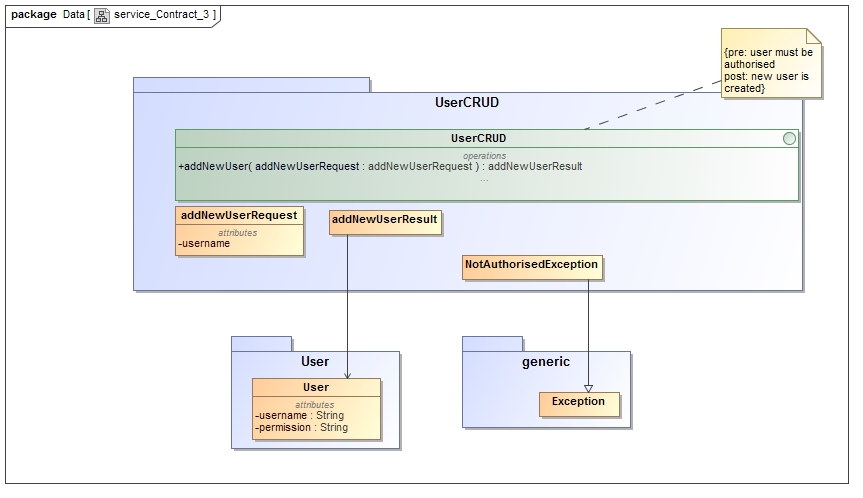
\includegraphics[width=1\linewidth]{./Graphics/4.jpg}
%\left(

%Change User Permissions
\subsection{Change user permissions}
\textbf{Description:}
This allows the administrator to promote or demote a user's access privilege.
\subsubsection{Prioritization:}
Important
\subsubsection{Conditions and Data Structures:}
\textbf{Pre-Conditions:}
	\begin{itemize}
	\item The user must be authorised to change the permissions
	\item The user, whose permission is being changed, must exist
	\end{itemize}
\textbf{Post-Conditions:}
	\begin{itemize}
	\item User's permissions is changed
	\end{itemize}	
%\subsubsection{Required Functionality:} 
%\subsubsection{Process Specifications:}
\subsubsection{Service contract:}
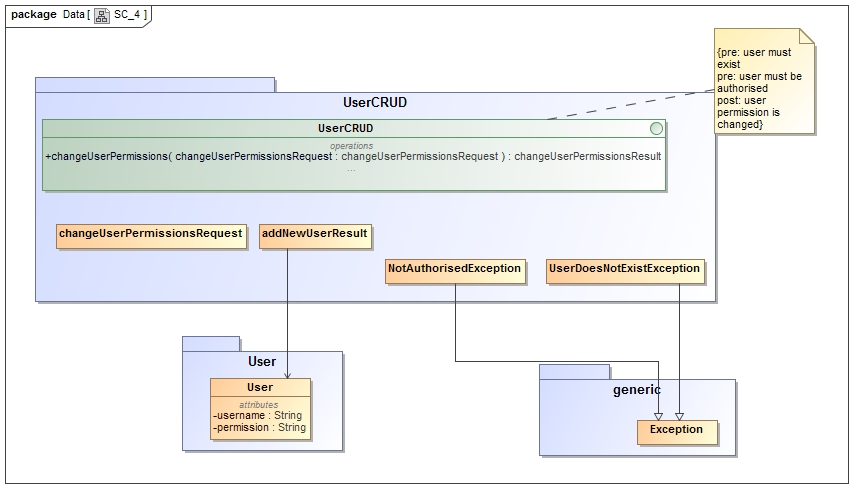
\includegraphics[width=1\linewidth]{./Graphics/5.jpg}
%\left(

%Delete
\subsection{Query All Patient Details}
\textbf{Description:}
This allows the administrator to remove a user from PIMS.
\subsubsection{Prioritization:}
Important
\subsubsection{Conditions and Data Structures:}
\textbf{Pre-Conditions:}
	\begin{itemize}
	\item The user must be authorised to remove users
	\item User must exist
	\end{itemize}
\textbf{Post-Conditions:}
	\begin{itemize}
	\item User is removed from PIMS.
	\end{itemize}	
%\subsubsection{Required Functionality:} 
%\subsubsection{Process Specifications:}
\subsubsection{Service contract:}
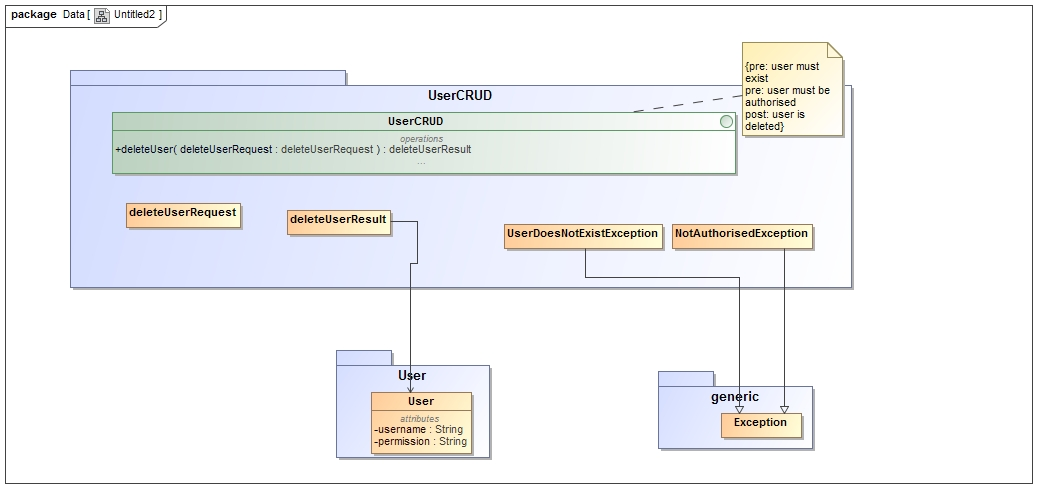
\includegraphics[width=1\linewidth]{./Graphics/6.jpg}
%\left(
